\subsection{UC2 - Visualizzazione Errore Interpretazione}
\begin{itemize}
    \item \textbf{Identificativo}: UC2
    \item \textbf{Nome}: Visualizzazione errore interpretazione
    \item \textbf{Descrizione grafica}:
\end{itemize}

\begin{figure}[h]
    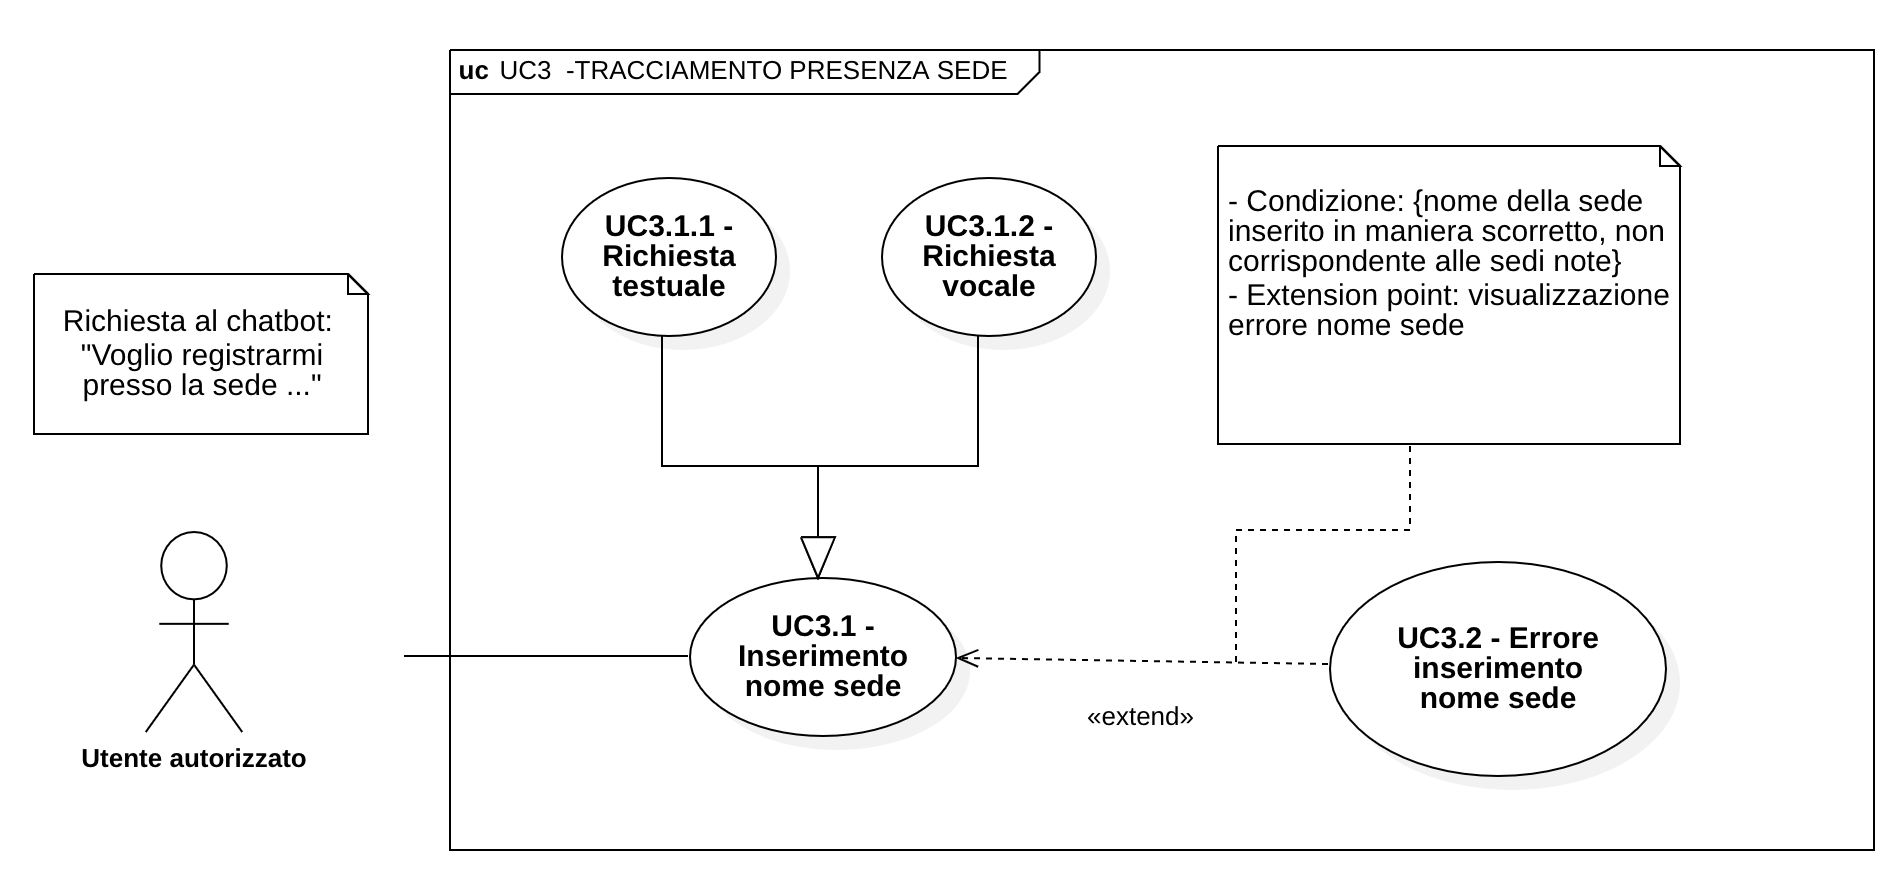
\includegraphics[scale=0.50]{images/UC2.png} 
    \caption{Diagramma UML del caso d'uso UC2 - Visualizzazione errore interpretazione}
\end{figure}

\begin{itemize}
    \item \textbf{Attori}:
    \begin{itemize} 
        \item \textit{Primari}: utente autorizzato
        \item \textit{Secondari}: non presenti
    \end{itemize}
 \item \textbf{Precondizione}: l'utente (precedentemente autenticato) sta scambiando una serie di messaggi con il chatbot (UC2.1.1) o (UC2.1.2) con lo scopo di eseguire una determinata azione.
 \item \textbf{Postcondizione}: il chatbot non è stato in grado di comprendere la richiesta dell'utente restituendo un messaggio di errore seguito da un insieme di comandi che è invece in grado di riconoscere.   
 \item \textbf{Scenario principale}: 
    \begin{itemize}
        \item Utente manda un messaggio al chatbot al fine di compire l'azione richiesta.
        \item Chatbot non è in grado di interpetare ciò che gli è stato chiesto.
        \item Chatbot restituisce un messaggio di errore e suggerisce alcuni comandi che l'utente può utilizzare.
    \end{itemize}
\end{itemize}
\newpage

\subsubsection{UC2.1 - Visualizzazione errore e suggerimento comandi}
\begin{itemize}
    \item \textbf{Identificativo}: UC2.1
    \item \textbf{Nome}: Visualizzazione errore e suggerimento comandi
    \item \textbf{Descrizione grafica}: (approfondita in UC2)
    \item \textbf{Attori}:
    \begin{itemize} 
        \item \textit{Primari}: utente autorizzato
        \item \textit{Secondari}: non presenti
    \end{itemize}
        \item \textbf{Precondizione}: il chatbot non è stato in grado di interpretare l'input fornito testualmente (UC2.1.1) oppure vocalmente (UC2.1.2), dall'utente (precedentemente) autenticato; verificandosi quindi una condizione di errore (UC2.2).
        \item \textbf{Postcondizione}: il chatbot mostra un messaggio di errore all'interno della chat e fornisce all'utente una serie di comandi che è in grado di interpretare in maniera corretta. 
     \item \textbf{Scenario principale}: 
        \begin{itemize}
            \item L'utente ha richiesto di eseguire un'operazione
            \item Chatbot non è in grado di interpetare ciò che gli è stato chiesto.
            \item Chatbot restituisce un messaggio di errore e suggerisce alcuni comandi che l'utente può utilizzare.
        \end{itemize}
\end{itemize}

\paragraph{UC2.1.1 - Richiesta testuale}
\begin{itemize}
    \item \textbf{Identificativo}: UC2.1.1
    \item \textbf{Nome}: Richiesta testuale
    \item \textbf{Descrizione grafica}: (approfondita in UC2)
    \item \textbf{Attori}:
    \begin{itemize} 
        \item \textit{Primari}: utente autorizzato
        \item \textit{Secondari}: non presenti
    \end{itemize}
        \item \textbf{Precondizione}: l'utente si è autenticato al sistema e vuole comunicare un messaggio al chatbot, in maniera testuale. 
        \item \textbf{Postcondizione}: l'utente fornisce un input testuale al chatbot. 
     \item \textbf{Scenario principale}: 
        \begin{itemize}
            \item L'utente ha effettuato l'accesso al sistema 
            \item L'utente fornisce un input testuale al chatbot 
        \end{itemize}
\end{itemize}

\paragraph{UC2.1.2 - Richiesta vocale}
\begin{itemize}
    \item \textbf{Identificativo}: UC2.1.2
    \item \textbf{Nome}: Richiesta vocale
    \item \textbf{Descrizione grafica}: (approfondita in UC2)
    \item \textbf{Attori}:
    \begin{itemize} 
        \item \textit{Primari}: utente autorizzato
        \item \textit{Secondari}: non presenti
    \end{itemize}
        \item \textbf{Precondizione}: l'utente si è autenticato al sistema e vuole comunicare un messaggio al chatbot, in maniera vocale. 
        \item \textbf{Postcondizione}: l'utente fornisce un input vocale al chatbot. 
     \item \textbf{Scenario principale}: 
        \begin{itemize}
            \item L'utente ha effettuato l'accesso al sistema 
            \item L'utente fornisce un input vocale al chatbot 
        \end{itemize}
\end{itemize}

\subsubsection{UC2.2 - Errore Interpretazione}
\begin{itemize}
    \item \textbf{Identificativo}: UC2.2
    \item \textbf{Nome}: errore interpretazione
    \item \textbf{Descrizione grafica}: (approfondita in UC2)
    \item \textbf{Attori}:
    \begin{itemize} 
        \item \textit{Primari}: utente autorizzato
        \item \textit{Secondari}: non presenti
    \end{itemize}
        \item \textbf{Precondizione}: l'utente ha fornito un input al chatbot, testuale (UC2.1.1) oppure vocale (UC2.1.2). 
        \item \textbf{Postcondizione}: il chatbot non è stato in grado di interpretare la richiesta dell'utente, vericando una condizione di errore. 
     \item \textbf{Scenario principale}: 
        \begin{itemize}
            \item Il chatbot ha ricevuto un input dall'utente che non è stato in grado di interpretare, causando un errore. 
        \end{itemize}
\end{itemize}


\newpage